\documentclass[tikz,border=2mm]{standalone}
\usepackage{luatex85}
\usepackage{fontspec}
\usepackage{xcolor}
% Color palette — single source of truth
% Loaded by preamble.tex and build/images/standalone-header.tex

\definecolor{trackone}{HTML}{1A6B6A}    % Track 1 (Confession) — deep teal
\definecolor{tracktwo}{HTML}{C4913B}    % Track 2 (Testament) — warm amber
\definecolor{trackthree}{HTML}{6B3FA0}  % Track 3 (Awakening) — violet
\definecolor{coverbg}{HTML}{0D1117}     % Cover background — near-black
\definecolor{textprimary}{HTML}{E6EDF3} % Text on dark backgrounds
\definecolor{phfill}{HTML}{D0D0D0}      % Placeholder fill — gray
\definecolor{bodytext}{HTML}{1A1A1A}    % Body text — near-black
\definecolor{linkblue}{HTML}{2563EB}    % Link color — accessible blue
\definecolor{trackconv}{HTML}{8C7853}   % Convergence (all tracks) — warm bronze
\definecolor{trackbridge}{HTML}{808080}  % Bridge (meta/hybrid) — neutral gray



\begin{document}
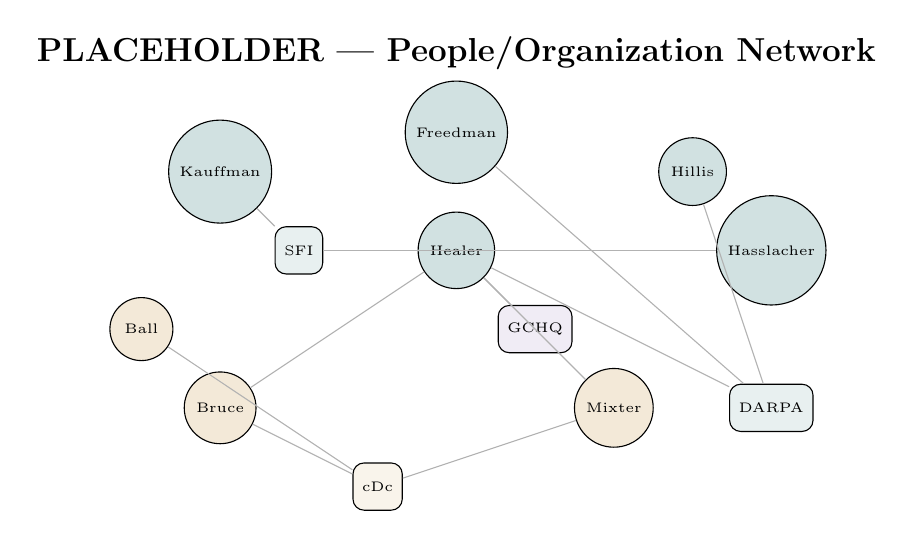
\begin{tikzpicture}[
  person/.style={circle, draw, minimum size=8mm, font=\tiny},
  org/.style={rectangle, draw, rounded corners, minimum height=6mm, font=\tiny},
  conn/.style={-, gray!60}
]

% Title
\node[font=\large\bfseries] at (0, 4.5) {PLACEHOLDER --- People/Organization Network};

% People
\node[person, fill=trackone!20] (healer) at (0, 2) {Healer};
\node[person, fill=tracktwo!20] (bruce) at (-3, 0) {Bruce};
\node[person, fill=trackone!20] (hillis) at (3, 3) {Hillis};
\node[person, fill=trackone!20] (kauffman) at (-3, 3) {Kauffman};
\node[person, fill=trackone!20] (freedman) at (0, 3.5) {Freedman};
\node[person, fill=tracktwo!20] (ball) at (-4, 1) {Ball};
\node[person, fill=trackone!20] (hasslacher) at (4, 2) {Hasslacher};
\node[person, fill=tracktwo!20] (mixter) at (2, 0) {Mixter};

% Organizations
\node[org, fill=trackone!10] (darpa) at (4, 0) {DARPA};
\node[org, fill=trackone!10] (sfi) at (-2, 2) {SFI};
\node[org, fill=trackthree!10] (gchq) at (1, 1) {GCHQ};
\node[org, fill=tracktwo!10] (cdc) at (-1, -1) {cDc};

% Connections
\draw[conn] (healer) -- (bruce);
\draw[conn] (healer) -- (gchq);
\draw[conn] (healer) -- (darpa);
\draw[conn] (healer) -- (mixter);
\draw[conn] (hillis) -- (darpa);
\draw[conn] (kauffman) -- (sfi);
\draw[conn] (hasslacher) -- (sfi);
\draw[conn] (freedman) -- (darpa);
\draw[conn] (ball) -- (cdc);
\draw[conn] (bruce) -- (cdc);
\draw[conn] (mixter) -- (cdc);
\draw[conn] (sfi) -- (healer);

\end{tikzpicture}
\end{document}
